\documentclass[10pt]{beamer}

\usetheme{glasgow}

\usepackage{booktabs}
\usepackage[scale=2]{ccicons}
\usepackage{minted}
\usepackage{bookmark}
\sisetup{per-mode=symbol,per-symbol = p}
\usepackage[style=verbose]{biblatex}
\renewcommand{\footnotesize}{\fontsize{5pt}{7pt}\selectfont}
% \usepackage{filecontents}% to embed the file `myreferences.bib` in your `.tex` file
% \begin{filecontents*}[noheader]{references.bib}
%     @book{rappaport_millimeter_2015,
% 	address = {Upper Saddle River, NJ},
% 	title = {Millimeter wave wireless communications},
% 	isbn = {978-0-13-217228-8},
% 	publisher = {Prentice Hall},
% 	author = {Rappaport, Theodore S. and Heath, Robert W. and Daniels, Robert C. and Murdock, James N.},
% 	year = {2015},
% 	keywords = {Millimeter wave communication systems, Wireless communication systems}
% }

% \addbibresource{references.bib}


% \usepackage[noadjust]{cite}
\usepgfplotslibrary{dateplot}

\usemintedstyle{trac}

% ($ (A)!r!(B) $) the location of images to be used
\graphicspath{{src/}}

%% Customisation
% \newcommand{\V}[1]{\v} % vectors \v{c}
% \renewcommand{\v}[1]{\mathbf{#1}} % vectors
\newcommand{\ti}[1]{\tilde{#1}} % spectral representation
\newcommand{\tnsr}[1]{\underline{\underline{#1}}}

% Symbols
\renewcommand{\O}{\omega}  % omega
\newcommand{\E}{\varepsilon}  % epsilon
\renewcommand{\u}{\mu}  % mu
\newcommand{\p}{\rho}  % rho
\newcommand{\x}{\times}  % times
\renewcommand{\inf}{\infty}  % infinity
\newcommand{\infint}{\int\limits_{-\inf}^\inf} % integral by R
\newcommand{\e}{\mathrm{e}} % Straight-up exponential
\renewcommand{\j}{{j}\mkern1mu} % Straight-up exponential
\newcommand{\iu}{\mathrm{i}\mkern1mu}

\newcommand\ddfrac[2]{\frac{\displaystyle #1}{\displaystyle #2}}

\usepackage{animate}



%     % Define a the counter cnt. Used to identify files generated for use
% % with Gnuplot.
% \newcounter{cnt}
% \setcounter{cnt}{0}

% % Macro for drawing one frame of the F-distribution animation.
% \newcommand{\fdst}[4]{%
%     % shade the critical region tail
%     \draw[fill,orange]  (#1,0) -- plot[id=5\thecnt,domain=#1:5.5,samples=50]
%         function {#4*(x**(0.5*#2-1))*((1+#2*x/#3)**(-0.5*#2-0.5*#3))}
%             -- (5.5,0) -- cycle;

%     % draw the F distribution curve
%     \draw[color=blue!50!black,thick]
%         plot[id=f4\thecnt,smooth,domain=0:5.5,samples=100]
%         function {#4*(x**(0.5*#2-1))*((1+#2*x/#3)**(-0.5*#2-0.5*#3))};

%     % draw the F axis
%     \draw[->] (0,0) -- (6,0) node[right] {$F$};
%     % label the critical region boundary
%     \draw (#1,0) -- (#1,-0.02) node[below] {$#1$};
%     % label 0
%     \draw (0,0) -- (0,-0.02) node[below] {$0$};

%     % add some lables for degrees of freedom and alpha level
%     \draw (2,0.5) node[right] {$df_1 = #2$};
%     \draw (2,0.4) node[right] {$df_2 = #3$};
%     \draw (2,0.3) node[right] {$\alpha = 0.10$};

%     % draw the y axis
%     \draw[very thin,->] (0,0) -- (0,0.8);
% }


\title{High Frequency Communication Systems}
\subtitle{Lecture 11}
\date{Spring 2021}
\author{Hasan T Abbas \& Qammer H Abbasi}
% \institute{}





\begin{document}

\maketitle

%%%%%%%%%%%%%%%%%%%%%%%%%%%%%%%%%%%%%%%%%%
%%%%%%%%%%%%%%%%%%%%%%%%%%%%%%%%%%%%%%%%%%
%%%%%%%%%%%%%%%%%%%%%%%%%%%%%%%%%%%%%%%%%%
\begin{frame}[fragile]
    \frametitle{Lecture Outline}
    \begin{outline}[itemize]
        \1 Terahertz Communications
        \1 Terahertz Generation
        \1 Plasmonics
        \1 Applications of Terahertz
    \end{outline}
\end{frame}
%%%%%%%%%%%%%%%%%%%%%%%%%%%%%%%%%%%%%%%%%%
%%%%%%%%%%%%%%%%%%%%%%%%%%%%%%%%%%%%%%%%%%
%%%%%%%%%%%%%%%%%%%%%%%%%%%%%%%%%%%%%%%%%%

\section{Terahertz Communications}

\begin{frame}
    \frametitle{The Terahertz Spectrum}
    \begin{columns}
        \normalsize
        \begin{column}{.6\textwidth}
            \begin{outline}
                \1 The electromagnetic (EM) spectrum between \SIrange{0.1}{10}{\THz} is called the \textit{THz band}.
                \1 Naturally, higher carrier frequency yields higher bandwidth
                \2 Not necessarily higher channel capacity
                \1 We can achieve bandwidths up to \SI{20}{Gbps}
                \2 A typical 8K movie requires \SI{200}{Mbps} bandwidth!
                \2 For comparison, optical fiber communication can provide \SI{39}{Tbps} bandwidth!
                \1 THz communications provide a promising application for backhauling of base stations
            \end{outline}
        \end{column}
        \begin{column}{.4\textwidth}
            \scriptsize
            \begin{figure}[T!]
                \centering
                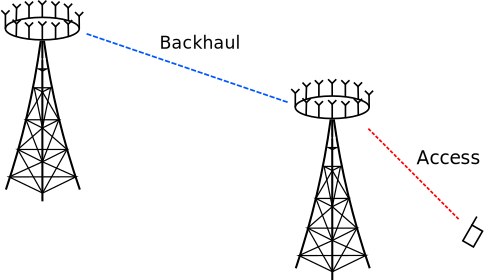
\includegraphics[width=.95\textwidth]{backhaul.pdf}
                \label{fig:backhaul_network}
            \end{figure}
        \end{column}
    \end{columns}
\end{frame}

\begin{frame}
    \frametitle{Terahertz Communications}

    \begin{figure}[h!]
        \centering
        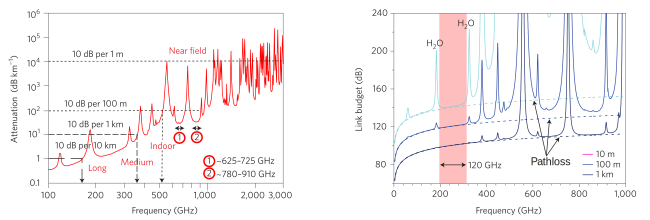
\includegraphics[width=.95\textwidth]{THz Attenuation.pdf}
        \caption{EM wave attenuation and free-space pathloss due to \ch{H20} molecules in the air in the THz spectrum \tiny{[Nagatsuma, T., \textit{et al}. Nature Photon 10, 371–379 (2016)]}.}
    \end{figure}
\end{frame}

\begin{frame}
    \frametitle{Terahertz Technology}
    \normalsize
    \begin{columns}
        \normalsize
        \begin{column}{.6\textwidth}
            \begin{outline}
                \1 Just like mmWave communications, THz waves have considerably high free-space pathloss
                \2 This requires even higher gain antennas ($\sim \SI{100}{\dB}$)
                \1 Current THz device technology does not allow us to increase the power levels
                \1 Since THz lies in the middle of microwave and optical frequencies, we get the \textit{best of both worlds}.
                \2 We have non-ionising waves
                \2 We can construct devices similar to optical technologies
            \end{outline}
        \end{column}
        \begin{column}{.44\textwidth}
            \scriptsize
            \begin{figure}
                \centering
                \includegraphics[width=.95\textwidth]{Scale.pdf}
                \label{fig:Terahertz_technology}
            \end{figure}
            \begin{figure}
                \centering
                \includegraphics[width=.95\textwidth]{sources_and_power.jpeg}
                \label{fig:sources_power}
            \end{figure}
        \end{column}
    \end{columns}

\end{frame}

\section{Terahertz Sources}


\begin{frame}
    \frametitle{Terahertz Generation}

    There are many ways to generate efficient THz signals. However, all the technologies have not fully developed to be widely available.
    \begin{figure}[h!]
        \centering
        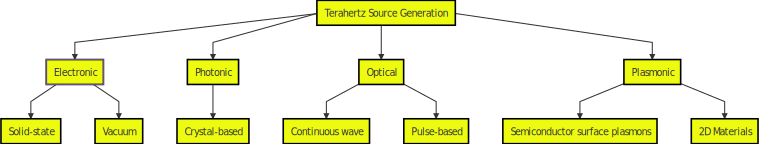
\includegraphics[width=1\textwidth]{terahertz_sources.pdf}
    \end{figure}
    Today, we will focus on the plasmonic technologies.
\end{frame}


\begin{frame}
    \frametitle{Terahertz Sources}

    \begin{figure}[h!]
        \centering
        \includegraphics[width=.75\textwidth]{Curto_resonator.pdf}
        \caption{Different Source techniques at THz and optical frequencies.}
    \end{figure}


\end{frame}

\begin{frame}
    \frametitle{Terahertz Sources - Extension of Microwave Technologies}
    \small
    \begin{outline}
        \1 Microwave based vacuum tube technologies are extended to THz frequencies
        \2 The process involves conversion of modulated electron current to electromagnetic radiation
        \2 These are often called \textit{fast-wave} devices
        \2 The phase velocity of the generated electromagnetic wave is greater than the speed of light
    \end{outline}
    \begin{figure}[h!]
        \centering
        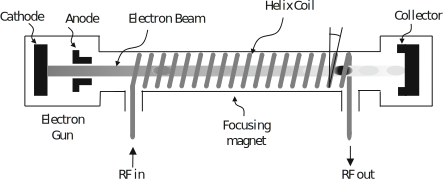
\includegraphics[width=.65\textwidth]{electron_gun.pdf}
        \caption{A typical vacuum-tube source \tiny{[Rieh, J-S.,  Intro to Terahertz Electronics, Springer (2021)]}.}
    \end{figure}
\end{frame}


\begin{frame}
    \frametitle{Photonic Terahertz Sources}
    \begin{figure}[t!]
        \centering
        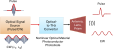
\includegraphics[width=.6\textwidth]{photonic_sources.pdf}
    \end{figure}
    \begin{outline}
        \1 The main idea is the optical-THz signal conversion through lasers
        \1 Non-linear optical (NLO) materials are used to generate \textit{monochromatic} THz waves
        \2 II-VI Semiconductor crystals such as \ch{ZnTe}, and \ch{CdTe} are commonly used as NLO materials
    \end{outline}
\end{frame}

\section{Plasmonics}

\begin{frame}
    \frametitle{Plasmonics Overview}
    % ----------------------------------------------------------
    \begin{columns} % align columns
        \begin{column}{.5\textwidth}
            \begin{outline}[itemize]
                \1 Interfacial wave phenomena
                \2 Metal-dielectric interface
                \2 Semiconductor heterostructure
                \1 Surface plasmon polaritons (SPPs)
            \end{outline}
            %
            \begin{outline}[itemize]
                \1 Plasma frequency
                \2 Metals - Optical frequency
                \2 Semiconductors - Terahertz
            \end{outline}
            %
        \end{column}
        \begin{column}{.5\textwidth}
            % Use this to preserve fonts from Inkspace
            \begin{figure}
                \centering
                \fontsize{6}{7}\selectfont% Reduce the fontsize
                \def\svgwidth{.8\linewidth}
                \input{src/spp.pdf_tex}
                \label{fig:spp}
                \caption{SPPs at optical frequencies}
            \end{figure}
            %
            \begin{figure}
                \centering
                \fontsize{6}{7}\selectfont
                \def\svgwidth{.8\linewidth}
                \input{src/spp_2deg.pdf_tex}
                \label{fig:spp_2deg}
                \caption{SPPs in the THz regime}
            \end{figure}
        \end{column}%
    \end{columns}
\end{frame}
% ------------------------------------------------------------
% ------------------------------------------------------------
% ------------------------------------------------------------
% ------------------------------------------------------------
% ------------------------------------------------------------
% ------------------------------------------------------------
% ------------------------------------------------------------
\begin{frame}
    \frametitle{Surface Plasmon Polaritons}

    \begin{columns} % align columns
        \begin{column}{.5\textwidth}
            \begin{minipage}[T][.1\textheight][c]{\linewidth}
                \begin{outline}[itemize]
                    \1 Slow surface waves
                    \1 Reduced Wavelength
                    \1 Focusing beyond the diffraction limit
                \end{outline}
                \begin{outline}[itemize]
                    \1 Optical SPP
                \end{outline}
                \setlength{\belowdisplayshortskip}{-7pt}
                \setlength{\abovedisplayshortskip}{2pt}
                \begin{equation} \nonumber
                    \Re \left[ \E_{\text{metal}}(\O)\right] < 0
                \end{equation}
                \begin{outline}[itemize]
                    \1 THz SPP
                \end{outline}
                \begin{equation} \nonumber
                    \Im \left[ \sigma_{s}(\O)\right] < 0
                \end{equation}
            \end{minipage}
        \end{column}
        \begin{column}{.5\textwidth}
            % Use this to preserve fonts from Inkspace
            \begin{figure}
                \centering \hspace*{-1.25cm}
                \fontsize{6}{7}\selectfont
                \def\svgwidth{1.1\linewidth}
                \input{src/spps_comp.pdf_tex}
                \label{fig:spp_2deg}
                \caption{Dispersion Curve comparison}
            \end{figure}
        \end{column}%
    \end{columns}
\end{frame}
% ------------------------------------------------------------
% ------------------------------------------------------------
% ------------------------------------------------------------
% ------------------------------------------------------------
% ------------------------------------------------------------
% ------------------------------------------------------------
% ------------------------------------------------------------
% ------------------------------------------------------------
\begin{frame}
    \frametitle{Nanoantennas}

    \begin{columns} % align columns
        \begin{column}{.4\textwidth}
            % \begin{minipage}[T][.1\textheight][c]{\linewidth}
            \vspace*{-1cm}
            \begin{outline}[itemize]
                \1 Convert Localized near-field to efficient far-field radiation
                \1 Low Q-factor
                \1 Extremely small size
                \1 \color{red}{High Purcell Factor}
            \end{outline}
            % \setlength{\belowdisplayshortskip}{-7pt}
            % \setlength{\abovedisplayshortskip}{2pt}
            \begin{equation} \nonumber
                {P}  = \frac{{Q}}{{V}}
            \end{equation}
            \begin{outline}[itemize]
                \1 Directive radiation
            \end{outline}
            % \end{minipage}
            %
        \end{column}
        %
        \begin{column}{.55\textwidth}
            % Use this to preserve fonts from Inkspace
            \begin{figure}
                \centering
                \fontsize{6}{7}\selectfont
                \def\svgwidth{1.0\linewidth}
                \input{src/curto.pdf_tex}
                \caption{Optical resonant cavities for electric field enhancement}
            \end{figure}
        \end{column}%
    \end{columns}
\end{frame}
%   % ------------------------------------------------------------
%   % ------------------------------------------------------------
%   % ------------------------------------------------------------
%   % ------------------------------------------------------------
%   % ------------------------------------------------------------
%   % ------------------------------------------------------------
%   % ------------------------------------------------------------
%   % ------------------------------------------------------------
\begin{frame}
    \frametitle{Nanoantennas}

    \begin{columns} % align columns
        \begin{column}{.45\textwidth}
            \begin{minipage}[T][.1\textheight][c]{\linewidth}
                \begin{outline}[itemize]
                    \1 Scaled-down microwave antenna designs
                    \1 Shift of resonance with width unlike in microwave regime
                \end{outline}
                \begin{figure}
                    \includegraphics[scale=.03]{bowtie_field_map.png}
                    % \caption{Subwavelength Transmission through a Silver slit}
                \end{figure}
            \end{minipage}
        \end{column}
        %
        \begin{column}{.55\textwidth}
            % Use this to preserve fonts from Inkspace
            \begin{figure}
                \centering
                \subfloat{\includegraphics[height = 1.4in]{generate_fig8c.tikz}
                    \label{fig:sim_his}}\\
                \centering
                \subfloat{\includegraphics[height = .8in]{fig8_a.png}
                    \label{fig:narrow}}
                \subfloat{\includegraphics[height = .8in]{fig8_d.png}
                    \label{fig:wide}}
                % \caption{(a) Maximum enhancement of a gold nanodipole excited at \SI{550}{\nm} (b) narrow and (c) wide profile. A narrow structure does not maintain resonance when widened without also changing its length.}
                \label{fig:simulationop}
            \end{figure}
        \end{column}%
    \end{columns}
\end{frame}
%     % ------------------------------------------------------------
%     % ------------------------------------------------------------
%     % ------------------------------------------------------------
%     % ------------------------------------------------------------
%     % ------------------------------------------------------------
%     % ------------------------------------------------------------
%     % ------------------------------------------------------------
%     % ------------------------------------------------------------
\begin{frame}
    \frametitle{Two-dimensional Electron Gas (2DEG)}

    \begin{columns} % align columns
        \begin{column}{.5\textwidth}
            \begin{minipage}[T][.1\textheight][c]{\linewidth}
                \begin{outline}[itemize]
                    \1 Semiconductor Heterostructure in high electron mobility transistor (HEMT)
                    \1 High concentration of free electrons ($\sim \num{1e11}-\SI{1e14}{\cm^{-2}}$)
                    \1 Very high Mobility ($\sim \num{1e3}-\SI{1e6}{\cm^{2}/V/s}$)
                    \1 Formation of Quantum Well
                    \2 Two-dimensional confinement of electrons
                \end{outline}
            \end{minipage}
            %
        \end{column}
        %
        \begin{column}{.5\textwidth}
            % Use this to preserve fonts from Inkspace
            \begin{figure}
                \centering
                \fontsize{6}{7}\selectfont
                \def\svgwidth{.8\linewidth}
                \input{src/hemt2.pdf_tex}
                \caption{Typical GaAs/AlGaAs HEMT}
            \end{figure}
            \begin{figure}
                \centering
                \fontsize{6}{7}\selectfont
                \def\svgwidth{.8\linewidth}
                \input{src/2deg_bandgap.pdf_tex}
                \caption{Band diagram of a GaAs/AlGaAs heterostructure}
            \end{figure}
        \end{column}%
    \end{columns}
\end{frame}
%       % ------------------------------------------------------------
%       % ------------------------------------------------------------
%       % ------------------------------------------------------------
%       % ------------------------------------------------------------
%       % ------------------------------------------------------------
%       % ------------------------------------------------------------
%       % ------------------------------------------------------------
%       % ------------------------------------------------------------
\begin{frame}
    \frametitle{2DEG (contd.)}

    \begin{columns} % align columns
        \begin{column}{.5\textwidth}
            \begin{minipage}[T][.1\textheight][c]{\linewidth}
                \begin{outline}[itemize]
                    \1 Plasma waves in 2DEG
                    \1 Dyakonov-Shur instability
                    \2 Voltage bias at source and drain terminals
                    \2 Plasma resonance
                    \2 THz emission
                    \1 Electronic Flute
                    \2 Tunable resonance with gate voltage
                \end{outline}
            \end{minipage}
            %
        \end{column}
        %
        \begin{column}{.5\textwidth}
            % Use this to preserve fonts from Inkspace
            \begin{figure}
                \fontsize{6}{7}\selectfont
                \def\svgwidth{1.1\linewidth}
                \input{src/flute_2deg2.pdf_tex}
                % \caption{Typical GaAs/AlGaAs HEMT}
            \end{figure}
            \begin{equation} \nonumber
                \begin{split}
                    \lambda &= \frac{c}{f} \\
                    & \Longrightarrow  300 \u \mathrm{m}
                \end{split}
                \label{eq:disp_TE_two}
            \end{equation}
        \end{column}%
    \end{columns}
\end{frame}

\begin{frame}
    \frametitle{SPP Dispersion Relation}
    \begin{columns}[T] % align columns
        \begin{column}{.5\textwidth}
            \begin{outline}[itemize]
                \1 SPP solution (pole expression)
            \end{outline}
            \begin{equation} \nonumber
                k_{sp}=\frac{\O}{c}\sqrt {\dfrac {\E_{1}\E_{2}(\O)} {\E_{1} + \E_{2}(\O)}}
                \label{eq:dis_spp}
            \end{equation}
            \begin{outline}[itemize]
                \1 Accurate material description
            \end{outline}
            \begin{equation} \nonumber
                \E_2(\O) = \E_{\inf} - \frac{\O_{d}^{2}}{\O^2 - \j\gamma \O} + \sum \limits_{i = 1}^N G_i(\O)
                \label{eq:eps_drude_cp}
            \end{equation}
            \begin{equation} \nonumber
                G_i(\O) = C_i \left[ \frac{e^{\j \phi_i}}{\O_i + \O - \j \Gamma_i} + \frac{e^{-\j \phi_i}}{\O_i - \O + \j \Gamma_i} \right]
                \label{eq:CP_terms}
            \end{equation}
        \end{column}
        \begin{column}[T]{.45\textwidth}
            \centering
            \begin{figure}
                \subfloat{\includegraphics[height = 1.25in]{ep_silver.tikz}
                    \label{fig:ep_gold}}

                \subfloat{\includegraphics[height = 1.25in]{disp_silver.tikz}
                    \label{fig:ep_silver}}
            \end{figure}
        \end{column}
    \end{columns}
\end{frame}


%     % ------------------------------------------------------------
%     % ------------------------------------------------------------
%     % ------------------------------------------------------------
%     % ------------------------------------------------------------
%     % ------------------------------------------------------------
%     % ------------------------------------------------------------
%     % ------------------------------------------------------------
\begin{frame}
    \frametitle{Theory and Methods}
    \frametitle{2DEG Circuit model}
    \begin{columns} % align columns
        \begin{column}{.5\textwidth}
            \begin{minipage}[T][.1\textheight][c]{\linewidth}
                \begin{outline}[itemize]
                    \1 Drude-Lorentz Surface Conductivity
                \end{outline}
                %
                \begin{equation} \nonumber
                    \sigma_s = \frac{N_s e^2}{m^{\ast}}\frac{\tau}{1 + \j \tau \O}
                    \label{eq:Y2deg}
                \end{equation}
                \begin{itemize}
                    \item[] {\makebox[.3cm][l]{$N_s$} - Surface charge density}
                    \item[] {\makebox[.3cm][l]{$\tau$} - Scattering time}
                    \item[] {\makebox[.3cm][l]{$m^{\ast}$} - Effective electron mass}
                \end{itemize}
                \begin{outline}[itemize]
                    \1 Equivalent Circuit
                \end{outline}
                \begin{equation} \nonumber
                    \sigma_s = \frac{1}{Z} = \frac{1}{R + {1}/{\j \O C}}
                    \label{eq:simga_TL}
                \end{equation}
            \end{minipage}
        \end{column}
        %
        \begin{column}{.5\textwidth}
            % Use this to preserve fonts from Inkspace
            \begin{figure}
                \includegraphics[height = 1.5in]{cond_2deg_gan.tikz}
                \label{fig:cond_2deg}
                \caption{Room temperature GaN/AlGaN 2DEG surface conductivity}
            \end{figure}
            %
            \begin{figure} \vspace*{-.75cm}
                \centering
                \fontsize{6}{7}\selectfont
                \def\svgwidth{.75\linewidth}
                \documentclass{standalone}
\usepackage{tikz}
\usepackage{circuitikz}
\usetikzlibrary{decorations.pathmorphing,%
decorations.pathreplacing,calc%
}
\usepackage{etoolbox}
\usepackage{physics}
\makeatletter

\pgfcircdeclarebipole{}
    {\ctikzvalof{bipoles/tline/height}}{tline}
    {\ctikzvalof{bipoles/tline/height}}
    {\ctikzvalof{bipoles/tline/width}}
{   
    %% First find distance from startpoint to endpoint
    \pgfpointdiff{\pgfpointanchor{\ctikzvalof{bipole/name}start}{center}}
                 {\pgfpointanchor{\ctikzvalof{bipole/name}end}{center}}
    \pgfmathparse{veclen(\the\pgf@x,\the\pgf@y)}
    %% The coordinate system has been changed so that the origin is at the midpoint and
    %% the line is along the x axis. So shift back by half the length of the line, and 
    %% make the cylinder of width roughly the length of the line, with a 40pt setback
    %% on each side.
    \pgftransformxshift{\pgfmathresult/2-30pt}
    \pgf@circ@res@left=\dimexpr-\pgfmathresult pt+40pt\relax
    %% Here is the original function, copied directly from the source of circuittikz, 
    %% down to next %%
    \pgf@circ@res@step=.2\pgf@circ@res@right % half x axis
    \pgfsetlinewidth{\pgfkeysvalueof{/tikz/circuitikz/bipoles/thickness}\pgfstartlinewidth}
    \pgfpathellipse{\pgfpoint{\pgf@circ@res@right-\pgf@circ@res@step}{0}}
                   {\pgfpoint{\pgf@circ@res@step}{0}}
                   {\pgfpoint{0}{-\pgf@circ@res@up}}
    \pgfpathmoveto{\pgfpoint{\pgf@circ@res@right-\pgf@circ@res@step}{\pgf@circ@res@up}}
    \pgfpathlineto{\pgfpoint{\pgf@circ@res@left+\pgf@circ@res@step}{\pgf@circ@res@up}}
    \pgfpatharc{-90}{90}{-\pgf@circ@res@step and -\pgf@circ@res@up}
    \pgfpathlineto{\pgfpoint{\pgf@circ@res@right-\pgf@circ@res@step}{\pgf@circ@res@down}}
    %% I have to fill the figure to block out the original line
    \pgfsetfillcolor{white}
    \pgfusepath{draw,fill}
    %% Redraw part of the line that gets blocked by the cylinder by mistake
    \pgfpathmoveto{\pgfpoint{\pgf@circ@res@right-2*\pgf@circ@res@step}{0pt}}
    \pgfpathlineto{\pgfpoint{\pgf@circ@res@right}{0pt}}
    \pgfusepath{draw}
}
\begin{document}
% \begin{tikzpicture}
% \end{tikzpicture}

\begin{circuitikz}[scale=1,
    interface/.style={postaction={draw, decorate, decoration={border,angle=45, amplitude=-3mm, segment length=2mm}}}
    ]
%% Transmission Line
\draw[-stealth,decorate,decoration={snake,amplitude=4pt,pre length=2pt,post length=1.5pt}] (-0.5,1) -- ++(2,0);
% \node (A) at (2,1) {$\va{E}, \va{H}$};
\node (A) at (-1,1) {$(V, I)$};

\draw (0,2) to[TL] (5,2);
\node (B) at (2.5,1) {$Z_{0,1},(\mu_1, \varepsilon_1)$};
\draw (0,0) to[TL] (5,0);
\draw (5,2) to[TL] (10,2);
\node (C) at (7.5,1) {$Z_{0,2}, (\mu_2, \varepsilon_2)$};
\draw (5,0) to[TL] (10,0);

\draw[dashed, thick, color=gray] (5,-1) to (5,6);

\draw[dashed, color=black] (-1,2) to (0,2);
\draw[dashed, color=black] (-1,0) to (0,0);

\draw[dashed, color=black] (10,2) to (11,2);
\draw[dashed, color=black] (10,0) to (11,0);

\draw[thick,->,color=black] (10,1) to (11,1);
\node (D) at (10.5,1.2) {$\vu{z}$};

%% Plane wave
\draw[-stealth,decorate,decoration={snake,amplitude=4pt,pre length=2pt,post length=1.5pt}] (-0.5,5) -- ++(2,0);
\node (A) at (-1,5) {$(\va{E}, \va{H})$};

\fill[gray!10] (5,2.5) rectangle (5.2,6.2);
\draw[gray,line width=.5pt,interface](5,3)--(5,6);
% \node (A) at (-1,1) {$(V, I)$};

\filldraw[fill=white, line width=1pt] (5,2) circle(0.9mm);
\filldraw[fill=white, line width=1pt] (5,0) circle(0.9mm);

\draw[thick,->,color=black] (5,6) to (6,6);
\node (E) at (5.6,6.2) {$\vu{z}$};

\draw[thick,->,color=black] (5,6) to (5,6.5);
\node (F) at (5,6.7) {$\vu{x}$};

\node (G) at (2.5,4.5) {$\eta_1$};
\node (H) at (7.5,4.5) {$\eta_2$};

\end{circuitikz}
\end{document} 
                % \caption{Typical GaAs/AlGaAs HEMT}
            \end{figure}
        \end{column}%
    \end{columns}
\end{frame}
%           % ------------------------------------------------------------
%           % ------------------------------------------------------------
%           % ------------------------------------------------------------
%           % ------------------------------------------------------------
%           % ------------------------------------------------------------
%           % ------------------------------------------------------------
%           % ------------------------------------------------------------
\begin{frame}
    \frametitle{Dispersion Relation for a 2D Sheet}
    \begin{columns}[T] % align columns
        \begin{column}{.5\textwidth}
            \begin{outline}[itemize]
                \1 Conductive Sheet in freespace
                \1 TM mode surface wave
            \end{outline}
            \begin{equation} \nonumber
                k^{\mathrm{TM}}_{\mathrm P} = \frac{\O}{c} \sqrt{1 - \left(\frac{2}{\eta_0 \sigma_s}\right)^2}
                \label{eq:TM_pole}%
            \end{equation}
            \begin{outline}[itemize]
                \1 Below plasma frequency
            \end{outline}
            \begin{equation} \nonumber
                \Im \sigma_s < 0
                \label{eq:2deg_surface_wave}%
            \end{equation}%
            \begin{outline}[itemize]
                \1 At low temperature
            \end{outline}%
            \begin{equation} \nonumber
                \Im |\sigma_s| \gg \Re |\sigma_s|
                \label{eq:2deg_low_loss}
            \end{equation}
        \end{column}
        \begin{column}[T]{.45\textwidth}
            \centering
            \begin{figure}
                \subfloat{\includegraphics[height = 1.25in]{disp_gaas_sheet_77.tikz}
                    \label{fig:disp_2deg_77}}

                \subfloat{\includegraphics[height = 1.25in]{disp_gaas_sheet_rt.tikz}
                    \label{fig:disp_2deg_rt}}
            \end{figure}
        \end{column}
    \end{columns}
\end{frame}

\section{Terahertz Applications}

\begin{frame}
    \frametitle{Terahertz Detection}
    Relying on the principle of reciprocity, we can use photoconductive antennas to detect THz radiation.
    \begin{figure}[h!]
        \centering
        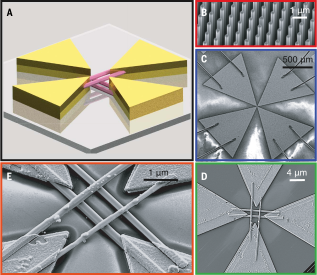
\includegraphics[width=.45\textwidth]{terahertz_applications.pdf}
        \caption{A polarisation sensitive cross-nanowire THz detector \tiny{[Peng et al., Science 368, 510–513 (2020)]}.}
    \end{figure}
\end{frame}

\begin{frame}
    \frametitle{Terahertz Imaging}
    \begin{outline}
        \1 THz waves have the ability to \textcolor{red}{see through} apparently opaque objects.
        \1 This is done in a non-ionising manner
        \1 Throug image processing, we can achieve high-resolution imaging through THz waves
    \end{outline}
    \begin{figure}[h!]
        \centering
        \includegraphics[width=.95\textwidth]{terahertz_imagin.png}
    \end{figure}
\end{frame}


\begin{frame}
    \frametitle{Material Characterisation}

    \small
    \begin{columns}
        \begin{column}{.4\textwidth}
            \begin{outline}
                \1 THz time-domain spectroscopy (THz-TDS) is a well-known method for charaterising the material properties of different substances
                \2 Attractive applications in explosives detection, counterfeit drug discovery and health monitoring of plants
                \1 Biggest feature is again, the non-ionising nature of THz waves
                \1 Common substances such as \ch{H2O} and \ch{N2} have strong absorption spectra
             \end{outline}
        \end{column}
        \begin{column}{.6\textwidth}
            \scriptsize
            \begin{figure}[T!]
                \centering
                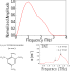
\includegraphics[width=.95\textwidth]{nitrogen.pdf}
                \label{fig:nitrogen}
            \end{figure}
        \end{column}
    \end{columns}
\end{frame}


\end{document}
